\documentclass[aspectratio=169,10pt]{beamer}
\usetheme{default}
\usepackage[T1]{fontenc}
\usepackage{lmodern}
\usepackage{listings}
\usepackage{upquote}
\usepackage{tabularx}
\usepackage{colortbl}
\usepackage{xcolor}
\usepackage{hyperref}
\usepackage{tikz}
\usetikzlibrary{positioning}
\definecolor{ink}{HTML}{10243A}
\definecolor{blue}{HTML}{1E6F9F}
\definecolor{teal}{HTML}{16A085}
\definecolor{amber}{HTML}{E5A23B}
\definecolor{paper}{HTML}{F4F7FA}
\definecolor{muted}{HTML}{607386}
\setbeamercolor{normal text}{fg=ink,bg=white}
\setbeamercolor{structure}{fg=blue}
\setbeamercolor{frametitle}{fg=white,bg=ink}
\setbeamercolor{title}{fg=white}
\setbeamercolor{block title}{fg=white,bg=blue}
\setbeamercolor{block body}{fg=ink,bg=paper}
\setbeamercolor{alertblock title}{fg=white,bg=amber}
\setbeamercolor{alertblock body}{fg=ink,bg=paper}
\setbeamercolor{exampleblock title}{fg=white,bg=teal}
\setbeamercolor{exampleblock body}{fg=ink,bg=paper}
\setbeamertemplate{blocks}[rounded][shadow=false]
\setbeamertemplate{navigation symbols}{}
\setbeamertemplate{footline}{\hfill\color{muted}\scriptsize Ubuntu Terminal Basics\hspace{1em}\insertframenumber\,/\,\inserttotalframenumber\hspace{1.2em}\vspace{0.7em}}
\setbeamertemplate{itemize item}{\color{teal}\scriptsize$\blacktriangleright$}
\setbeamertemplate{itemize subitem}{\color{amber}\tiny$\bullet$}
\lstdefinestyle{terminal}{
  basicstyle=\ttfamily\small,
  backgroundcolor=\color{ink},
  basicstyle=\color{white}\ttfamily\small,
  keywordstyle=\color{white},
  commentstyle=\color{teal!50},
  frame=single, rulecolor=\color{ink},
  showstringspaces=false, breaklines=true,
  columns=fullflexible, keepspaces=true,
  xleftmargin=0.6em, xrightmargin=0.6em,
  aboveskip=0.6em, belowskip=0.6em
}
\lstset{style=terminal}
\newcommand{\key}[1]{\fcolorbox{blue!30}{paper}{\strut\texttt{#1}}}
\newcommand{\term}[1]{\texttt{#1}}
\newenvironment{hintblock}{\setbeamercolor{block title}{fg=ink,bg=teal!22}\setbeamercolor{block body}{fg=ink,bg=teal!5}\begin{block}{Hint}}{\end{block}}
\newenvironment{warningbox}[1]{\setbeamercolor{block title}{fg=ink,bg=amber!38}\setbeamercolor{block body}{fg=ink,bg=amber!10}\begin{block}{Warning: #1}}{\end{block}}
\title{Ubuntu Terminal Basics}
\subtitle{A practical first tour of the Linux terminal}
\author{Dr. Kaveh Hooshmandi}
\date{}
\begin{document}

\begin{frame}[plain]
  \begin{tikzpicture}[remember picture,overlay]
    \fill[ink] (current page.south west) rectangle (current page.north east);
    \fill[blue] (current page.south east) -- ++(-4.2,0) -- ++(4.2,3.2) -- cycle;
    \fill[teal] (current page.north east) -- ++(-2.1,0) -- ++(2.1,-1.7) -- cycle;
  \end{tikzpicture}
  \vspace{1.3cm}
  {\color{white}\Huge\bfseries Ubuntu Terminal Basics\par}
  \vspace{0.35cm}
  {\color{white!78}\Large A practical first tour of the Linux terminal\par}
  \vspace{0.6cm}
  {\color{white!65}\normalsize Chapter 1 \quad|\quad Ubuntu command line essentials\par}
  \vspace{0.65cm}
  {\color{white}\large\bfseries Dr. Kaveh Hooshmandi\par}
  \vspace{0.12cm}
  {\color{white!85}\small Primary academic email: \texttt{k.hooshmandi@arakut.ac.ir}\par}
  {\color{white!70}\small Secondary email: \texttt{Hooshmandi.kaveh@gmail.com}\par}
\end{frame}

\begin{frame}{What you will learn}
  \begin{columns}[T,onlytextwidth]
    \column{.56\textwidth}
      \begin{itemize}
        \item Why the terminal is useful for repeatable work
        \item Navigate folders and create, inspect, and remove files
        \item Redirect command output and use Tab completion
        \item Recognize when elevated permissions can cause damage
        \item Open the current folder in Ubuntu's file manager
      \end{itemize}
    \column{.40\textwidth}
      \begin{block}{One simple idea}
        The terminal is a direct way to ask Ubuntu to do a task. Learn a few small commands, then reuse them throughout the course.
      \end{block}
  \end{columns}
\end{frame}

\begin{frame}[fragile]{First terminal examples (1/2): write and read}
  \begin{lstlisting}
mkdir -p ~/terminal_practice
cd ~/terminal_practice
echo "Hello" > test.txt
cat test.txt
echo "first line" > test.txt
echo "second line" >> test.txt
cat test.txt
  \end{lstlisting}
  \begin{columns}[T,onlytextwidth]
    \column{.48\textwidth}
      \begin{block}{What the symbols mean}
        \term{>} (create or replace a file)\\[3pt]
        \term{\textgreater\kern0pt\textgreater} (append to the end of a file)
      \end{block}
    \column{.48\textwidth}
      \begin{exampleblock}{Check the result}
        The first \term{cat test.txt} prints \term{Hello}. The last one prints \term{first line} and \term{second line} on separate lines.
      \end{exampleblock}
  \end{columns}
\end{frame}

\begin{frame}[fragile]{First terminal examples (2/2): files and Python}
  \begin{lstlisting}
ls > files.txt
cat files.txt
xdg-open .
printf 'print("Hello from Python")\n' > test.py
python3 test.py
cd ~/
  \end{lstlisting}
  \begin{columns}[T,onlytextwidth]
    \column{.48\textwidth}
      \begin{block}{Paths and programs}
        \term{.} (current folder)\\[3pt]
        \term{\textasciitilde{}/} (your home folder)\\[3pt]
        \term{python3 test.py} (run the script)
      \end{block}
    \column{.48\textwidth}
      \begin{warningbox}{Root shell}
        A root shell (administrator session) is not needed for these exercises. Work in your own practice folder.
      \end{warningbox}
  \end{columns}
\end{frame}

\section{Why the terminal?}
\begin{frame}{1.1 \; Who cares about the terminal?}
  \begin{columns}[T,onlytextwidth]
    \column{.58\textwidth}
      \begin{itemize}
        \item It gives a consistent way to describe steps in a tutorial.
        \item Commands are easy to repeat, share, and adapt.
        \item Development tools are often launched and inspected from a shell.
      \end{itemize}
      \vspace{0.25cm}
      \alert{You do not need to become a terminal expert today.}
    \column{.38\textwidth}
      \begin{block}{Think of it as a tool}
        A graphical interface is great for many tasks. The terminal complements it when exact, repeatable commands are useful.
      \end{block}
  \end{columns}
\end{frame}

\section{The terminal}
\begin{frame}{1.2 \; The terminal: a command workspace}
  \begin{columns}[T,onlytextwidth]
    \column{.43\textwidth}
      \begin{hintblock}
        Open a terminal with \key{Ctrl+Alt+T}. The shell reads a command, runs it, then shows the result and a new prompt.
      \end{hintblock}
      \begin{exampleblock}{Command shape}
        \centering\term{command} \; \term{option} \; \term{target}\\[3pt]
        \raggedright Example: \term{ls -l \textasciitilde{}/Documents}
      \end{exampleblock}
    \column{.54\textwidth}
      \begin{block}{Useful command families}
        \small
        \begin{tabular}{@{}p{.14\linewidth}p{.78\linewidth}@{}}
          \term{pwd}, \term{ls} & Find where you are and see files\\
          \term{cd}, \term{mkdir} & Move between folders; create folders\\
          \term{touch}, \term{cat} & Create an empty file; read its contents\\
          \term{grep} & Show lines containing a word\\
          \term{nano} & Edit a text file in the terminal\\
          \term{apt}, \term{sudo} & Install software; request admin rights\\
          \term{alias} & Give a frequently used command a short name
        \end{tabular}
      \end{block}
  \end{columns}
\end{frame}

\begin{frame}{1.2 \; Useful command line programs (1/2)}
  \normalsize
  \renewcommand{\arraystretch}{1.15}
  \begin{block}{Table 1 -- the book's command toolkit, with teaching examples}
    \begin{tabularx}{\linewidth}{@{}>{\bfseries\ttfamily}p{1.65cm}>{\ttfamily}p{4cm}X@{}}
      \rowcolor{blue!13}\normalfont\bfseries Command & \normalfont\bfseries Example & \normalfont\bfseries What to expect\\
      pwd & pwd & Prints the full path of your current folder.\\[3pt]
      mkdir & mkdir a\_folder & Creates a new folder here.\\[3pt]
      cd & cd a\_folder & Moves the shell into that folder.\\[3pt]
      touch & touch a\_file.txt & Creates an empty file, or updates its timestamp.\\[3pt]
      cat & cat a\_file.txt & Prints the contents of a text file.\\[3pt]
      rm & rm a\_file.txt & Deletes a file; \texttt{-r} also removes a directory tree.\\
    \end{tabularx}
  \end{block}
  \begin{warningbox}{Know your location before \term{rm}}
    Run \term{pwd} and \term{ls} first. A deleted file normally does not go to the Trash.
  \end{warningbox}
\end{frame}

\begin{frame}{1.2 \; Useful command line programs (2/2)}
  \normalsize
  \renewcommand{\arraystretch}{1.15}
  \begin{block}{Table 1 -- continued}
    \begin{tabularx}{\linewidth}{@{}>{\bfseries\ttfamily}p{1.65cm}>{\ttfamily}p{4cm}X@{}}
      \rowcolor{blue!13}\normalfont\bfseries Command & \normalfont\bfseries Example & \normalfont\bfseries What to expect\\
      ls & ls & Lists files and folders.\\[3pt]
      grep & cat a\_file.txt \textbar{} grep robot & Keeps lines that contain \term{robot}.\\[3pt]
      nano & nano a\_file.txt & Opens a simple terminal text editor.\\[3pt]
      sudo & sudo apt update & Runs a command with administrator rights.\\[3pt]
      apt & sudo apt install git & Installs an Ubuntu package (after repository setup).\\[3pt]
      alias & alias hi="echo hello" & Creates a short name for a command in this shell.\\
    \end{tabularx}
  \end{block}
  \begin{hintblock}
    This table contains all 12 programs in the source chapter. The following slides show how to use them in practice.
  \end{hintblock}
\end{frame}

\begin{frame}{How a terminal command gets work done}
  \centering
  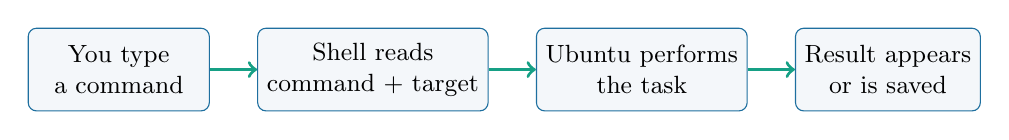
\begin{tikzpicture}[node distance=.6cm, every node/.style={font=\small},
    box/.style={draw=blue,fill=paper,rounded corners=3pt,minimum width=2.3cm,minimum height=1.05cm,align=center},
    arr/.style={->,very thick,teal}]
    \node[box] (you) {You type\\a command};
    \node[box,right=of you] (shell) {Shell reads\\command + target};
    \node[box,right=of shell] (ubuntu) {Ubuntu performs\\the task};
    \node[box,right=of ubuntu] (result) {Result appears\\or is saved};
    \draw[arr] (you)--(shell); \draw[arr] (shell)--(ubuntu); \draw[arr] (ubuntu)--(result);
  \end{tikzpicture}
  \vspace{0.55cm}
  \begin{columns}[T,onlytextwidth]
    \column{.48\textwidth}
      \begin{exampleblock}{Example: ask for your location}
        Type \term{pwd}. Ubuntu prints the full path of the current folder.
      \end{exampleblock}
    \column{.48\textwidth}
      \begin{hintblock}
        Most commands finish and return a prompt. A running program can be stopped with \key{Ctrl+C}.
      \end{hintblock}
  \end{columns}
\end{frame}

\begin{frame}[fragile]{Search text and reuse a command}
  \begin{block}{Find matching names with \term{grep}}
    \begin{lstlisting}
ls | grep notes
    \end{lstlisting}
    \term{ls} lists filenames; the pipe passes them to \term{grep}, which keeps names containing \term{notes}.
  \end{block}
  \begin{exampleblock}{Create a short alias}
    \begin{lstlisting}
alias hi='echo hello'
hi
    \end{lstlisting}
    \term{alias} gives a command a short name in the current shell session.
  \end{exampleblock}
  \begin{hintblock}
    A pipe \term{|} connects one command's output to the next command's input.
  \end{hintblock}
\end{frame}

\section{Let's use it}
\begin{frame}[fragile]{1.3 \; Let's use it (!?) -- make a practice folder}
  \begin{lstlisting}
# Move to your home folder, then create a workspace for this exercise
cd ~
mkdir terminal_practice
cd terminal_practice
touch empty.txt
pwd
ls
  \end{lstlisting}
  \begin{columns}[T,onlytextwidth]
    \column{.50\textwidth}
      \begin{hintblock}
        \term{\textasciitilde} means your home folder. \term{.} means the folder you are in now.
      \end{hintblock}
    \column{.47\textwidth}
      \begin{exampleblock}{What should you see?}
        \term{pwd} ends in \term{/terminal\_practice}; \term{ls} lists \term{empty.txt}. The prompt returns after each command.
      \end{exampleblock}
  \end{columns}
\end{frame}

\begin{frame}{Folders are locations: read the path}
  \centering
  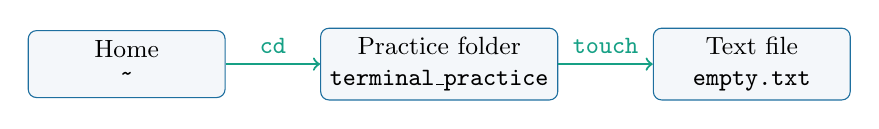
\begin{tikzpicture}[every node/.style={font=\small},
    folder/.style={draw=blue,fill=paper,rounded corners=3pt,minimum width=2.5cm,minimum height=.85cm,align=center},
    link/.style={->,thick,teal}]
    \node[folder] (home) {Home\\\term{\textasciitilde}};
    \node[folder,right=1.2cm of home] (practice) {Practice folder\\\term{terminal\_practice}};
    \node[folder,right=1.2cm of practice] (file) {Text file\\\term{empty.txt}};
    \draw[link] (home)--node[above]{\term{cd}} (practice);
    \draw[link] (practice)--node[above]{\term{touch}} (file);
  \end{tikzpicture}
  \vspace{.5cm}
  \begin{block}{Absolute path vs. current location}
    \term{/home/your-name/terminal\_practice} describes the full route. After \term{cd terminal\_practice}, the shorter name works because that folder is now the current location.
  \end{block}
  \begin{alertblock}{Check before changing files}
    Run \term{pwd} to confirm your location and \term{ls} to inspect its contents.
  \end{alertblock}
\end{frame}

\begin{frame}[fragile]{Create, edit, and read a text file}
  \begin{columns}[T,onlytextwidth]
    \column{.48\textwidth}
      \begin{lstlisting}
nano notes.txt
      \end{lstlisting}
      Type a short line, then save and exit Nano:
      \begin{enumerate}
        \item \key{Ctrl+X}
        \item \key{Y} to save
        \item \key{Enter} to confirm the filename
      \end{enumerate}
    \column{.48\textwidth}
      \begin{lstlisting}
cat notes.txt
ls
      \end{lstlisting}
      \begin{exampleblock}{What to expect}
        \term{cat notes.txt} prints the line you saved. \term{ls} lists \term{notes.txt} in the current folder.
      \end{exampleblock}
  \end{columns}
\end{frame}

\begin{frame}[fragile]{Terminal keyboard shortcuts}
  \begin{columns}[T,onlytextwidth]
    \column{.48\textwidth}
      \begin{block}{Copy and paste in a terminal}
        Copy selected text: \key{Ctrl+Shift+C}\\[5pt]
        Paste text: \key{Ctrl+Shift+V}
      \end{block}
      \begin{hintblock}
        Nano displays shortcuts along the bottom. Its symbol \term{\textasciicircum X} means \key{Ctrl+X}.
      \end{hintblock}
    \column{.48\textwidth}
      \begin{block}{Stop a running command}
        \begin{lstlisting}
sleep 30
        \end{lstlisting}
        Press \key{Ctrl+C} to stop it and return to the prompt.
      \end{block}
  \end{columns}
\end{frame}

\begin{frame}[fragile,shrink=5]{Clean up the practice folder carefully}
  \begin{warningbox}{Pause before using \term{rm}}
    Files removed with \term{rm} do not go to the Trash. Check the path and target first.
  \end{warningbox}
  \vspace{-0.24cm}
  \begin{lstlisting}
# Go back home, then remove only the practice folder from this example
cd ~
  rm -r terminal_practice
  \end{lstlisting}
  \vspace{-0.12cm}
  \begin{itemize}
    \item Use \term{ls} and \term{pwd} to verify your location.
    \item Never paste an unfamiliar destructive command without understanding its target.
  \end{itemize}
\end{frame}

\section{Bash redirections}
\begin{frame}[fragile]{1.4 \; Bash redirections: save command output}
  \begin{hintblock}
    Before writing a script for a small, common task, check whether Bash already has a simple command for it.
  \end{hintblock}
  \begin{center}
    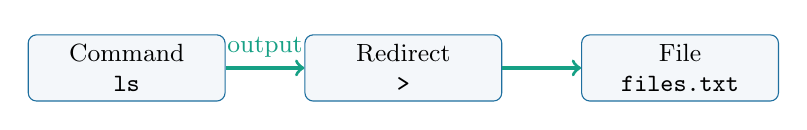
\begin{tikzpicture}[every node/.style={font=\small},
      box/.style={draw=blue,fill=paper,rounded corners=3pt,minimum width=2.5cm,minimum height=.72cm,align=center},
      arrow/.style={->,very thick,teal}]
      \node[box] (cmd) {Command\\\term{ls}};
      \node[box,right=1.0cm of cmd] (op) {Redirect\\\term{>}};
      \node[box,right=1.0cm of op] (dest) {File\\\term{files.txt}};
      \draw[arrow] (cmd)--node[above]{output} (op); \draw[arrow] (op)--(dest);
    \end{tikzpicture}
  \end{center}
  \begin{columns}[T,onlytextwidth]
    \column{.48\textwidth}
      \begin{exampleblock}{Replace: \term{>}}
        \term{ls > files.txt} saves the listing. Creates the file if needed; replaces old contents if it already exists.
      \end{exampleblock}
    \column{.48\textwidth}
      \begin{exampleblock}{Add: \term{\textgreater\kern0pt\textgreater}}
        \term{echo "done" \textgreater\kern0pt\textgreater files.txt} adds a line at the end and keeps existing contents.
      \end{exampleblock}
  \end{columns}
  \begin{warningbox}{Check the operator before pressing Enter}
    \term{>} overwrites the target file immediately; \term{\textgreater\kern0pt\textgreater} appends to it.
  \end{warningbox}
\end{frame}

\section{Tab completion}
\begin{frame}[fragile]{1.5 \; Tab completion: type less, check more}
  \begin{columns}[T,onlytextwidth]
    \column{.48\textwidth}
      \begin{block}{Try it}
        \begin{enumerate}
          \item Type \term{cd \textasciitilde{}} and press Enter.
          \item Type \term{ls} to see the available names.
          \item Start a command, such as \term{cat result\_}.
          \item Press \key{Tab} to complete a unique match.
        \end{enumerate}
      \end{block}
    \column{.48\textwidth}
      \begin{exampleblock}{If more than one name matches}
        Press \key{Tab} twice to display possible matches. Add another letter or two, then press Tab again.
      \end{exampleblock}
      \begin{hintblock}
        Tab completion works for commands, folders, and files. Use it often to avoid long-path typos.
      \end{hintblock}
  \end{columns}
\end{frame}

\section{Safety and permissions}
\begin{frame}{1.6 \; Be careful with \term{sudo}}
  \begin{warningbox}{Use elevated privileges only when needed}
    \term{sudo} runs a command with administrator privileges. A mistake can affect the whole system.
  \end{warningbox}
  \begin{itemize}
    \item In this course, use \term{sudo} for system-wide package installation when instructed.
    \item Do not add \term{sudo} just to make an error message disappear.
    \item Read the command and its target before entering your password.
  \end{itemize}
  \begin{exampleblock}{Expected course pattern}
    A package installation may need \term{sudo apt install ...}; ordinary work in your project folder should not.
  \end{exampleblock}
\end{frame}

\begin{frame}{1.7 \; Be careful even without \term{sudo}}
  \centering
  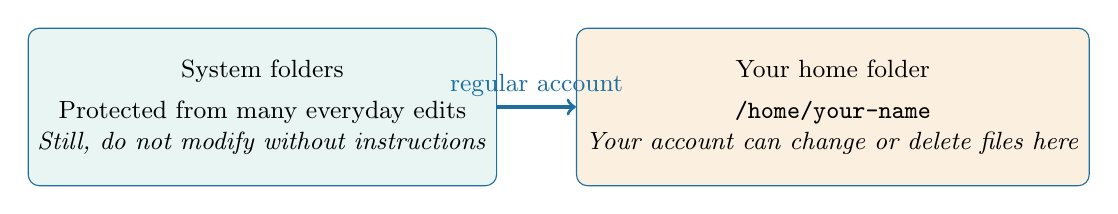
\begin{tikzpicture}[every node/.style={font=\small},
    area/.style={draw=blue,rounded corners=4pt,minimum width=4.6cm,minimum height=2cm,align=center},
    safe/.style={area,fill=teal!10}, personal/.style={area,fill=amber!16}]
    \node[safe] (system) {System folders\\[4pt]Protected from many everyday edits\\\textit{Still, do not modify without instructions}};
    \node[personal,right=1cm of system] (home) {Your home folder\\[4pt]\term{/home/your-name}\\\textit{Your account can change or delete files here}};
    \draw[->,very thick,blue] (system)--node[above]{regular account} (home);
  \end{tikzpicture}
  \vspace{0.45cm}
  \begin{warningbox}{Your home folder is yours to change}
    \term{rm} does not need \term{sudo} to delete files you own. Before a change, check the target with \term{pwd} and \term{ls}.
  \end{warningbox}
\end{frame}

\begin{frame}{1.8 \; File permissions: leave system ownership alone}
  \centering
  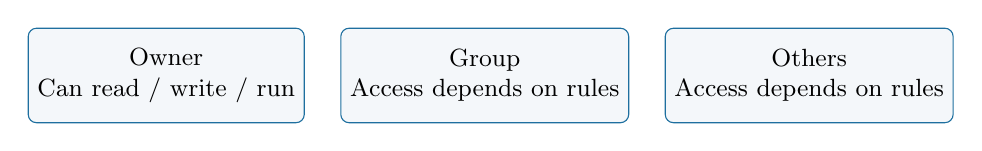
\begin{tikzpicture}[every node/.style={font=\small},
    role/.style={draw=blue,fill=paper,rounded corners=3pt,minimum width=2.65cm,minimum height=1.2cm,align=center}]
    \node[role] (owner) {Owner\\Can read / write / run};
    \node[role,right=.45cm of owner] (group) {Group\\Access depends on rules};
    \node[role,right=.45cm of group] (other) {Others\\Access depends on rules};
  \end{tikzpicture}
  \vspace{.45cm}
  \begin{itemize}
    \item Permissions decide who may read, change, or run a file.
    \item Saving a file as administrator may make it owned by the administrator account.
    \item Then your normal account may be unable to edit it or launch desktop tools that need it.
  \end{itemize}
  \begin{warningbox}{Beginner rule}
    Avoid experimenting with \term{chmod} (change permissions), \term{chown} (change ownership), or administrator-mode editors. Follow a specific, trusted instruction if a permission change is ever required.
  \end{warningbox}
\end{frame}

\section{Nautilus}
\begin{frame}[fragile]{1.9 \; Nautilus: browse files with a GUI}
  \begin{columns}[T,onlytextwidth]
    \column{.45\textwidth}
      \begin{itemize}
        \item Nautilus is Ubuntu's default file manager, similar to File Explorer or Finder.
        \item Open the folder you are already working in, then use the visual browser to inspect files.
      \end{itemize}
      \begin{hintblock}
        The dot \term{.} is a path shortcut for the current folder.
      \end{hintblock}
    \column{.52\textwidth}
      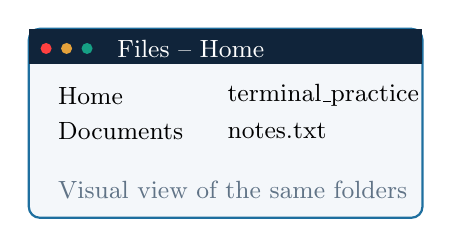
\begin{tikzpicture}[every node/.style={font=\small}]
        \draw[rounded corners=4pt,thick,blue,fill=paper] (0,0) rectangle (5,2.4);
        \fill[ink] (0,1.95) rectangle (5,2.4);
        \fill[red!75] (.22,2.15) circle (.07); \fill[amber] (.48,2.15) circle (.07); \fill[teal] (.74,2.15) circle (.07);
        \node[anchor=west,text=white] at (1,2.15) {Files -- Home};
        \node[anchor=west] at (.25,1.55) {Home};
        \node[anchor=west] at (.25,1.1) {Documents};
        \node[anchor=west] at (2.4,1.55) {terminal\_practice};
        \node[anchor=west] at (2.4,1.1) {notes.txt};
        \node[anchor=west,color=muted] at (.25,.35) {Visual view of the same folders};
      \end{tikzpicture}
      \begin{lstlisting}
cd ~
nautilus .
      \end{lstlisting}
      \small \term{cd \textasciitilde{}} moves to Home; \term{nautilus .} opens it in the file browser.
  \end{columns}
\end{frame}

\section{Linux workflow for development}
\begin{frame}[fragile]{A repeatable Linux workflow}
  \begin{center}
    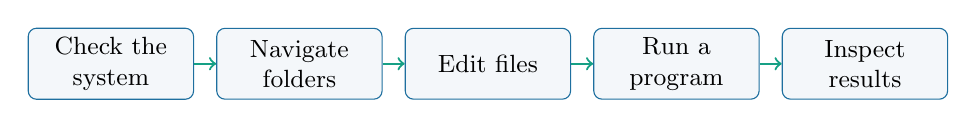
\begin{tikzpicture}[every node/.style={font=\small},
      stagebox/.style={draw=blue,fill=paper,rounded corners=3pt,minimum width=2.1cm,minimum height=.9cm,align=center},
      arrow/.style={->,thick,teal}]
      \node[stagebox] (start) {Check the\\system};
      \node[stagebox,right=.28cm of start] (navigate) {Navigate\\folders};
      \node[stagebox,right=.28cm of navigate] (edit) {Edit files};
      \node[stagebox,right=.28cm of edit] (run) {Run a\\program};
      \node[stagebox,right=.28cm of run] (inspect) {Inspect\\results};
      \draw[arrow] (start)--(navigate); \draw[arrow] (navigate)--(edit);
      \draw[arrow] (edit)--(run); \draw[arrow] (run)--(inspect);
    \end{tikzpicture}
  \end{center}
  \begin{lstlisting}
mkdir -p ~/linux_lab/src
cd ~/linux_lab
pwd
  \end{lstlisting}
  \begin{hintblock}
    This creates a safe practice folder in your Home directory. In the following examples, \term{linux\_lab} is your own small project.
  \end{hintblock}
\end{frame}

\begin{frame}[fragile]{Identify the system and get help}
  \begin{lstlisting}
cat /etc/os-release  # distribution and version
echo "$SHELL"        # login shell
command -v python3  # path to a program
python3 --help       # program options
man ls               # detailed manual; q quits
  \end{lstlisting}
  \begin{block}{Read the answer}
    \term{command -v python3} prints the executable path if Python is installed. If a command is unknown, check its spelling, installation, and shell \term{PATH}.
  \end{block}
  \begin{exampleblock}{Try this}
    Compare \term{ls --help} with \term{man ls}. Find the option for showing hidden files.
  \end{exampleblock}
\end{frame}

\begin{frame}[fragile]{Paths: absolute, relative, and special names}
  \begin{lstlisting}
cd ~/linux_lab/src  # home-relative path
pwd                 # absolute path, starting with /
cd ..               # move to parent folder
cd .                # stay in current folder
cd ~                # return home
  \end{lstlisting}
  \begin{columns}[T,onlytextwidth]
    \column{.48\textwidth}
      \begin{block}{Absolute path}
        Starts with \term{/}. Example: \term{/home/student/linux\_lab/src} identifies the same place from anywhere.
      \end{block}
    \column{.48\textwidth}
      \begin{hintblock}
        \term{.} means here; \term{..} means parent; \term{\textasciitilde{}} means your Home directory.
      \end{hintblock}
  \end{columns}
\end{frame}

\begin{frame}[fragile]{Create, copy, move, and remove files}
  \begin{lstlisting}
cd ~/linux_lab
touch notes.txt
cp notes.txt notes_copy.txt  # duplicate a file
mv notes_copy.txt old.txt    # rename or move a file
ls
rm old.txt                 # remove only this practice file
  \end{lstlisting}
  \begin{block}{Predict the listing}
    Before \term{rm}, \term{ls} shows \term{notes.txt}, \term{old.txt}, and \term{src}. After \term{rm}, \term{old.txt} is gone.
  \end{block}
  \begin{warningbox}{Check the exact target}
    \term{rm} acts immediately. Use \term{pwd} and \term{ls} before removal. A directory needs \term{rm -r}; never use that option casually.
  \end{warningbox}
\end{frame}

\begin{frame}[fragile]{Read and search text files}
  \begin{lstlisting}
printf 'alpha\nbeta\nalpha again\n' > ~/linux_lab/notes.txt
cat ~/linux_lab/notes.txt
grep 'alpha' ~/linux_lab/notes.txt
wc -l ~/linux_lab/notes.txt
less ~/linux_lab/notes.txt  # press q to quit
  \end{lstlisting}
  \begin{exampleblock}{Expected result}
    \term{grep} returns two matching lines; \term{wc -l} reports three lines. \term{less} lets you scroll through a longer file.
  \end{exampleblock}
  \begin{hintblock}
    \term{head -n 5 file.txt} shows the first five lines; \term{tail -n 5 file.txt} shows the last five.
  \end{hintblock}
\end{frame}

\begin{frame}[fragile]{Find files and use patterns carefully}
  \begin{lstlisting}
cd ~/linux_lab
find . -name '*.txt'       # search this tree
ls *.txt                   # list matching names here
grep -R 'alpha' .          # search text in this tree
  \end{lstlisting}
  \begin{block}{What the star means}
    In \term{ls *.txt}, Bash expands \term{*.txt} to matching filenames before \term{ls} runs. In \term{find}, the quoted pattern is passed to the program.
  \end{block}
  \begin{warningbox}{Inspect a pattern before deletion}
    First run \term{ls *.txt}. Then, if you really mean every match, use a command that changes files. Patterns can match more than you expect.
  \end{warningbox}
\end{frame}

\begin{frame}[fragile]{Quote paths and arguments with spaces}
  \begin{lstlisting}
mkdir -p ~/linux_lab/'My Files'
touch ~/linux_lab/'My Files'/report.txt
cd ~/linux_lab/'My Files'
pwd
  \end{lstlisting}
  \begin{block}{Why quotes matter}
    Without quotes, Bash treats \term{My} and \term{Files} as separate arguments. The single quotes keep them together as one path.
  \end{block}
  \begin{hintblock}
    Tab completion can insert the needed escape characters for a filename with spaces.
  \end{hintblock}
\end{frame}

\begin{frame}[fragile]{Install Ubuntu packages with \term{apt}}
  \begin{lstlisting}
sudo apt update      # refresh package lists
apt search git       # search available packages
apt show git         # inspect version and description
sudo apt install git # install the selected package
  \end{lstlisting}
  \begin{block}{Understand the sequence}
    \term{update} refreshes the package index; \term{install} changes the system. \term{sudo} is needed for system package changes, so read the package name first.
  \end{block}
  \begin{hintblock}
    \term{apt list --installed git} checks whether \term{git} is installed. Package availability depends on configured repositories.
  \end{hintblock}
\end{frame}

\begin{frame}[fragile]{Environment variables: settings in a shell}
  \begin{lstlisting}
echo "$HOME"                        # home directory
echo "$PATH"                        # program search path
export PROJECT_DIR="$HOME/linux_lab" # set a variable
echo "$PROJECT_DIR"
printenv | grep PROJECT_DIR
  \end{lstlisting}
  \begin{block}{What changed?}
    \term{export} makes \term{PROJECT\_DIR} available to programs started by this shell. A separate terminal does not inherit changes made afterward in this one.
  \end{block}
  \begin{hintblock}
    Quotes around \term{"\$PROJECT\_DIR"} keep a value containing spaces together as one argument.
  \end{hintblock}
\end{frame}

\begin{frame}[fragile]{\term{source} and \term{.bashrc}: current vs. new shells}
  \begin{lstlisting}
cd ~/linux_lab
printf 'export DEMO_MODE=ready\n' > demo_env.sh
source ./demo_env.sh
echo "$DEMO_MODE"  # expected: ready
  \end{lstlisting}
  \begin{block}{Why \term{source} is different}
    It runs the script in the current shell, so the variable remains available there. Running the script as a separate process would not modify the parent shell.
  \end{block}
  \begin{hintblock}
    Bash reads \term{\textasciitilde{}/.bashrc} when an interactive shell opens. Put only intentional, reviewed startup commands in it.
  \end{hintblock}
\end{frame}

\begin{frame}[fragile]{Permissions: read, write, and execute}
  \begin{lstlisting}
cd ~/linux_lab
printf '#!/usr/bin/env bash\necho ready\n' > check.sh
ls -l check.sh
chmod u+x check.sh
./check.sh              # expected: ready
  \end{lstlisting}
  \begin{block}{Read \term{chmod u+x}}
    \term{u} means the file's owner; \term{+x} adds execute permission for that owner. \term{./check.sh} runs the script in the current folder.
  \end{block}
  \begin{warningbox}{Make only the needed change}
    Avoid \term{chmod 777} and arbitrary \term{chown} commands. Inspect \term{ls -l} and the error message first.
  \end{warningbox}
\end{frame}

\begin{frame}[fragile]{Processes: start, observe, and stop}
  \begin{lstlisting}
sleep 30          # runs in the foreground; Ctrl+C stops it
sleep 30 &        # runs in the background
jobs              # show shell jobs
kill %1           # stop job 1 from this shell
  \end{lstlisting}
  \begin{block}{Foreground vs. background}
    A foreground command occupies the terminal until it ends or you stop it. A trailing \term{\&} returns the prompt while the command runs.
  \end{block}
  \begin{hintblock}
    \term{ps -ef | grep sleep} can help find a process. A new terminal has its own job list.
  \end{hintblock}
\end{frame}

\begin{frame}[fragile]{Pipes and redirections: route program output}
  \begin{lstlisting}
cd ~/linux_lab
ls | sort             # send output into another command
ls > files.txt        # create or replace a file
ls >> files.txt       # append to the file
ls | tee listing.txt  # show and save at the same time
  \end{lstlisting}
  \begin{columns}[T,onlytextwidth]
    \column{.48\textwidth}
      \begin{block}{Read from left to right}
        The pipe \term{|} connects two commands. \term{sort} receives the names printed by \term{ls}.
      \end{block}
    \column{.48\textwidth}
      \begin{warningbox}{\term{>} replaces data}
        It does not ask before overwriting an existing file. \term{\textgreater\kern0pt\textgreater} adds lines instead.
      \end{warningbox}
  \end{columns}
\end{frame}

\begin{frame}[fragile]{Errors and logs: capture evidence}
  \begin{lstlisting}
cd ~/linux_lab
ls missing.txt 2> errors.log  # save error output
cat errors.log
tail -n 10 errors.log       # last ten lines
  \end{lstlisting}
  \begin{block}{Two output streams}
    Normal output goes to standard output; error messages go to standard error. \term{2>} redirects errors to a file, while \term{>} redirects normal output.
  \end{block}
  \begin{hintblock}
    \term{tail -f app.log} follows a growing log. Press \key{Ctrl+C} to stop following it.
  \end{hintblock}
\end{frame}

\begin{frame}[fragile]{Git: track changes in a project folder}
  \begin{lstlisting}
cd ~/linux_lab
git init
printf '# Linux lab\n' > README.md
git status
git add README.md
git status
  \end{lstlisting}
  \begin{block}{What to observe}
    The first \term{git status} shows an untracked file. After \term{git add}, it shows the file staged. No commit is made in this example.
  \end{block}
  \begin{hintblock}
    When using someone else's repository, read its README and check the branch before editing or building.
  \end{hintblock}
\end{frame}

\begin{frame}[fragile]{Python projects: isolate dependencies}
  \begin{lstlisting}
cd ~/linux_lab
python3 --version
python3 -m venv .venv
source .venv/bin/activate
python -m pip --version
deactivate
  \end{lstlisting}
  \begin{block}{What activation changes}
    The active shell uses the project's Python and \term{pip}. \term{deactivate} returns to the prior environment. The folder \term{.venv/} belongs to this project.
  \end{block}
  \begin{hintblock}
    If \term{venv} is unavailable, inspect the Ubuntu package \term{python3-venv}. Install packages only after checking the project's instructions.
  \end{hintblock}
\end{frame}

\begin{frame}[fragile]{Network basics: inspect, then test}
  \begin{lstlisting}
hostname             # this machine's name
hostname -I          # local IP addresses
ip -brief address    # interfaces and addresses
ping -c 3 127.0.0.1  # test the local network stack
  \end{lstlisting}
  \begin{block}{What these commands tell you}
    An address identifies a network interface. The loopback address \term{127.0.0.1} reaches this computer only; it does not test another machine.
  \end{block}
  \begin{hintblock}
    When two machines must communicate, record both addresses and verify each can reach the other before debugging the application.
  \end{hintblock}
\end{frame}

\begin{frame}[fragile]{Device files: inspect access before changing it}
  \begin{lstlisting}
ls /dev/ttyUSB*       # list matching serial devices, if any
ls -l /dev/ttyUSB0    # owner, group, and permissions
groups                # your account's groups
  \end{lstlisting}
  \begin{block}{Why device files matter}
    USB serial adapters and other hardware may appear under \term{/dev}. A program must have permission to open the relevant device file.
  \end{block}
  \begin{warningbox}{Use the hardware instructions}
    The correct group or \term{udev} rule depends on the device. Avoid broad permission changes; inspect the device first.
  \end{warningbox}
\end{frame}

\begin{frame}{Troubleshooting: start from the symptom}
  \begin{tabularx}{\textwidth}{@{}p{4cm}X@{}}
    \rowcolor{blue!13}\bfseries Symptom & \bfseries First useful command\\[3pt]
    Command not found & \term{command -v name}; check installation and \term{PATH}.\\[6pt]
    File not found & \term{pwd}, \term{ls}, then \term{find . -name 'file'}.\\[6pt]
    Permission denied & \term{ls -l file}; inspect owner and group.\\[6pt]
    Program seems stuck & \term{ps -ef}; identify the process, then use \key{Ctrl+C} for a foreground program.\\[6pt]
    Unexpected output & Capture error text with \term{2> errors.log}; read it with \term{cat} or \term{less}.\\
  \end{tabularx}
  \vspace{.3cm}
  \begin{hintblock}
    Record the exact command, folder, and first error message. That evidence usually points to the next check.
  \end{hintblock}
\end{frame}

\begin{frame}[fragile]{Mini lab: one small project from start to result}
  \begin{lstlisting}
mkdir -p ~/linux_lab/src
cd ~/linux_lab
printf 'print("hello from Linux")\n' > src/hello.py
python3 src/hello.py | tee run.log
grep 'hello' run.log
ls -lah src run.log
  \end{lstlisting}
  \begin{block}{Expected result}
    Python prints \term{hello from Linux}; \term{tee} saves the same line in \term{run.log}; \term{grep} finds that line. \term{ls} confirms the script and log exist.
  \end{block}
  \begin{exampleblock}{Explain each step}
    Which command created a folder? Which wrote a file? Which ran a program? Which showed and saved the result?
  \end{exampleblock}
\end{frame}

\begin{frame}{Linux readiness checklist}
  \begin{enumerate}
    \item I can check my Ubuntu version and get command help: \term{cat /etc/os-release}, \term{--help}.
    \item I can navigate and inspect files: \term{pwd}, \term{cd}, \term{ls}, \term{find}.
    \item I can edit, search, and route text: \term{nano}, \term{grep}, \term{|}, \term{>}, \term{tee}.
    \item I can install an Ubuntu package with \term{apt} when needed.
    \item I understand shell variables, \term{source}, and \term{\textasciitilde{}/.bashrc}.
    \item I can inspect permissions, a process, a log, and a device file.
    \item I can create and run the mini lab script and explain its output.
  \end{enumerate}
\end{frame}

\begin{frame}[shrink=2]{Practice check: can you explain each command?}
  \begin{block}{Read first, then predict what happens}
    \centering\term{cd \textasciitilde{}} \;\(\rightarrow\)\; \term{mkdir demo} \;\(\rightarrow\)\; \term{cd demo} \;\(\rightarrow\)\; \term{touch note.txt} \;\(\rightarrow\)\; \term{ls}
  \end{block}
  \begin{enumerate}
    \item Which command moves you to the home folder?
    \item What does \term{touch} do in this example?
    \item What should \term{ls} display?
    \item Which operator appends output: \term{>} or \term{\textgreater\kern0pt\textgreater}?
    \item Why should you check the target before running \term{rm -r}?
  \end{enumerate}
  \begin{exampleblock}{Expected result}
    \term{ls} should show \term{note.txt}. The \term{\textgreater\kern0pt\textgreater} operator appends. \term{rm -r} can permanently remove its target, so inspect the path and name first.
  \end{exampleblock}
\end{frame}

\begin{frame}{Quick recap}
  \begin{center}
    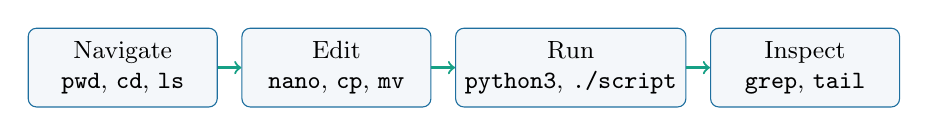
\begin{tikzpicture}[every node/.style={font=\small},
      summary/.style={draw=blue,fill=paper,rounded corners=3pt,minimum width=2.4cm,minimum height=1cm,align=center},
      arrow/.style={->,thick,teal}]
      \node[summary] (navigate) {Navigate\\\term{pwd}, \term{cd}, \term{ls}};
      \node[summary,right=.3cm of navigate] (prepare) {Edit\\\term{nano}, \term{cp}, \term{mv}};
      \node[summary,right=.3cm of prepare] (run) {Run\\\term{python3}, \term{./script}};
      \node[summary,right=.3cm of run] (inspect) {Inspect\\\term{grep}, \term{tail}};
      \draw[arrow] (navigate)--(prepare); \draw[arrow] (prepare)--(run); \draw[arrow] (run)--(inspect);
    \end{tikzpicture}
  \end{center}
  \begin{itemize}
    \item Confirm paths and file targets before editing, redirecting, or deleting.
    \item Use \term{apt} for system packages and a project environment for local Python dependencies.
    \item Remember that each terminal has its own variables and running jobs; use \key{Ctrl+C} to stop a foreground command.
    \item Diagnose failures through error text, logs, paths, processes, and permissions.
  \end{itemize}
\end{frame}

\begin{frame}{Sources and next reading}
  \begin{block}{Chapter basis}
    Sections 1.1--1.9 and the twelve-command table are adapted from the supplied \emph{Ubuntu Terminal Basics} chapter.
  \end{block}
  \begin{block}{Built-in references}
    Try \term{man bash}, \term{man ls}, \term{man chmod}, and a program's \term{--help} option.\\[4pt]
    The file and script exercises use the \term{\textasciitilde{}/linux\_lab} practice folder; package management is shown separately.
  \end{block}
  \begin{hintblock}
    Read each command and its expected effect before running it, especially commands that install packages or remove files.
  \end{hintblock}
\end{frame}

\begin{frame}{Presenter and contact}
  \begin{center}
    {\Large\bfseries Dr. Kaveh Hooshmandi}\par
  \end{center}
  \vspace{0.25cm}
  \begin{block}{Primary academic email}
    \href{mailto:k.hooshmandi@arakut.ac.ir}{\texttt{k.hooshmandi@arakut.ac.ir}}
  \end{block}
  \begin{block}{Additional email}
    \href{mailto:Hooshmandi.kaveh@gmail.com}{\texttt{Hooshmandi.kaveh@gmail.com}}
  \end{block}
\end{frame}

\end{document}
